%\documentclass[a4paper]{article}
\usepackage[utf8]{inputenc}
\usepackage[spanish, es-tabla, es-noshorthands]{babel}
\usepackage[table,xcdraw]{xcolor}
\usepackage[a4paper, footnotesep=1.25cm, headheight=1.25cm, top=2.54cm, left=2.54cm, bottom=2.54cm, right=2.54cm]{geometry}
%\geometry{showframe}

%\usepackage{wrapfig}			%Wrap figure in text
\usepackage[export]{adjustbox}	%Move images
\usepackage{changepage}			%Move tables

\usepackage{tikz}
\usepackage{amsmath}
\usepackage{amsfonts}
\usepackage{amssymb}
\usepackage{float}
\usepackage{graphicx}
\usepackage{caption}
\usepackage{subcaption}
\usepackage{multicol}
\usepackage{multirow}
\usepackage{wrapfig}
\setlength{\doublerulesep}{\arrayrulewidth}
\usepackage{booktabs}
\usepackage[numbib, nottoc, notlot, notlof]{tocbibind}

\usepackage{hyperref}
\hypersetup{
    colorlinks=true,
    linkcolor=blue,
    filecolor=magenta,      
    urlcolor=blue,
    citecolor=blue,    
}

%Change Font Size

% #1 = size, #2 = text
\newcommand{\setparagraphsize}[2]{{\fontsize{#1}{6}\selectfont#2 \par}}		%Cambia el size de todo el parrafo
\newcommand{\setlinesize}[2]{{\fontsize{#1}{6}\selectfont#2}}				%Cambia el font de una oración

\newcommand{\note}[1]{
	\begin{center}
		\huge{ \textcolor{red}{#1} }
	\end{center}
}

%FONTS (IMPORTANTE): Compilar en XeLaTex o LuaLaTeX
\usepackage{anyfontsize}	%Font size
\usepackage{fontspec}		%Font type

\usepackage{etoolbox}
\usepackage{todonotes}

\newcommand{\observacion}[2]{  \ifnumequal{1}{#1}{ { \todo[inline,backgroundcolor=red!25,bordercolor=red!100]{\textbf{Observación: #2}} } }{  }  }

\setcounter{topnumber}{2}
\setcounter{bottomnumber}{2}
\setcounter{totalnumber}{4}
\renewcommand{\topfraction}{0.85}
\renewcommand{\bottomfraction}{0.85}
\renewcommand{\textfraction}{0.15}
\renewcommand{\floatpagefraction}{0.8}
\renewcommand{\textfraction}{0.1}
\setlength{\floatsep}{5pt plus 2pt minus 2pt}
\setlength{\textfloatsep}{5pt plus 2pt minus 2pt}
\setlength{\intextsep}{5pt plus 2pt minus 2pt}

\newcommand{\quotes}[1]{``#1''}
\usepackage{array}
\newcolumntype{C}[1]{>{\centering\let\newline\\\arraybackslash\hspace{0pt}}m{#1}}
\usepackage[american]{circuitikz}
\usetikzlibrary{calc}
\usepackage{fancyhdr}
\usepackage{units} 

\graphicspath{{../Control de posición no lineal/}{../Control de fuerza no lineal/}{../Control híbrido no lineal/}{../Referencias/}{../Deducción de modelo/}{../Conclusiones/}}

\pagestyle{fancy}
\fancyhf{}
\lhead{22.99 - Automación Industrial}
\rhead{Lambertucci, Londero B., Maselli, Mechoulam}
\rfoot{Página \thepage}

%Items con bullets y no cuadrados
\renewcommand{\labelitemi}{\textbullet }

%
%\begin{document}

Para el modelado de la planta, se tomaron las ecuaciones provistas del libro de Astrom y Murray:

%\begin{equation}
%	\begin{pmatrix}
%		\dot{x_1} \\
%		\dot{x_2} \\
%		\dot{x_3} \\
%		\dot{x_4} 
%	\end{pmatrix} =
%	\begin{pmatrix}
%		x_2 \\
%		x_4 \\
%		\frac{-m l sin(x_3) {x_4}^2 + mg \left[ \frac{m l^2}{J_t} cos(x_3) sin(x_3) + F \right] }{M_t - m \left[ \frac{m l^2}{J_t} {cos(x_3)}^2 \right]} \\
%	\frac{-m l^2 sin(x_3) cos(x_3) {x_4}^2 + M_t g l sin(x_3) + l cos(x_3) F}{\frac{J_t M_t}{m} - m \left[l cos(x_3)\right]^2}
%	\end{pmatrix}
%\end{equation}

\begin{equation}
\label{eq:aym}
\begin{gathered}
	\dot{x_1} = x_2
	\\
	\dot{x_2} = x_4
	\\
	\dot{x_3} = \frac{-m l sin(x_3) {x_4}^2 + mg \left[ \frac{m l^2}{J_t} cos(x_3) sin(x_3) + F \right] }{M_t - m \left[ \frac{m l^2}{J_t} {cos(x_3)}^2 \right]}
	\\
	\dot{x_4} = \frac{-m l^2 sin(x_3) cos(x_3) {x_4}^2 + M_t g l sin(x_3) + l cos(x_3) F}{\frac{J_t M_t}{m} - m \left[l cos(x_3)\right]^2}
\end{gathered}
\end{equation}

Donde:
\begin{multicols}{2}
\begin{itemize}
	\item La masa del carro es $M = 0.5 \ kg$.
	\item La masa del péndulo es $m = 0.2 \ kg$.
	%\item La fricción es $b = 0$.
	\item La inercia es $J = 0.006 \ kg \cdot m^2$.
	\item La gravedad es $g = 9.8 \ \nicefrac{m}{s^2}$.
	\item El largo del péndulo es $L = 0.6 \ m$.
	\item La distancia la centro de masa del péndulo $l = 0.3 \ m$.
	\item $M_t = M + m$.
	\item $J_t = J + m l^2$.
\end{itemize}
\end{multicols}

Para el desarrollo en Simulink se valió del sistema presente en la Figura (\ref{fig:planta_simscape}).

\begin{figure}[H]
	\centering
	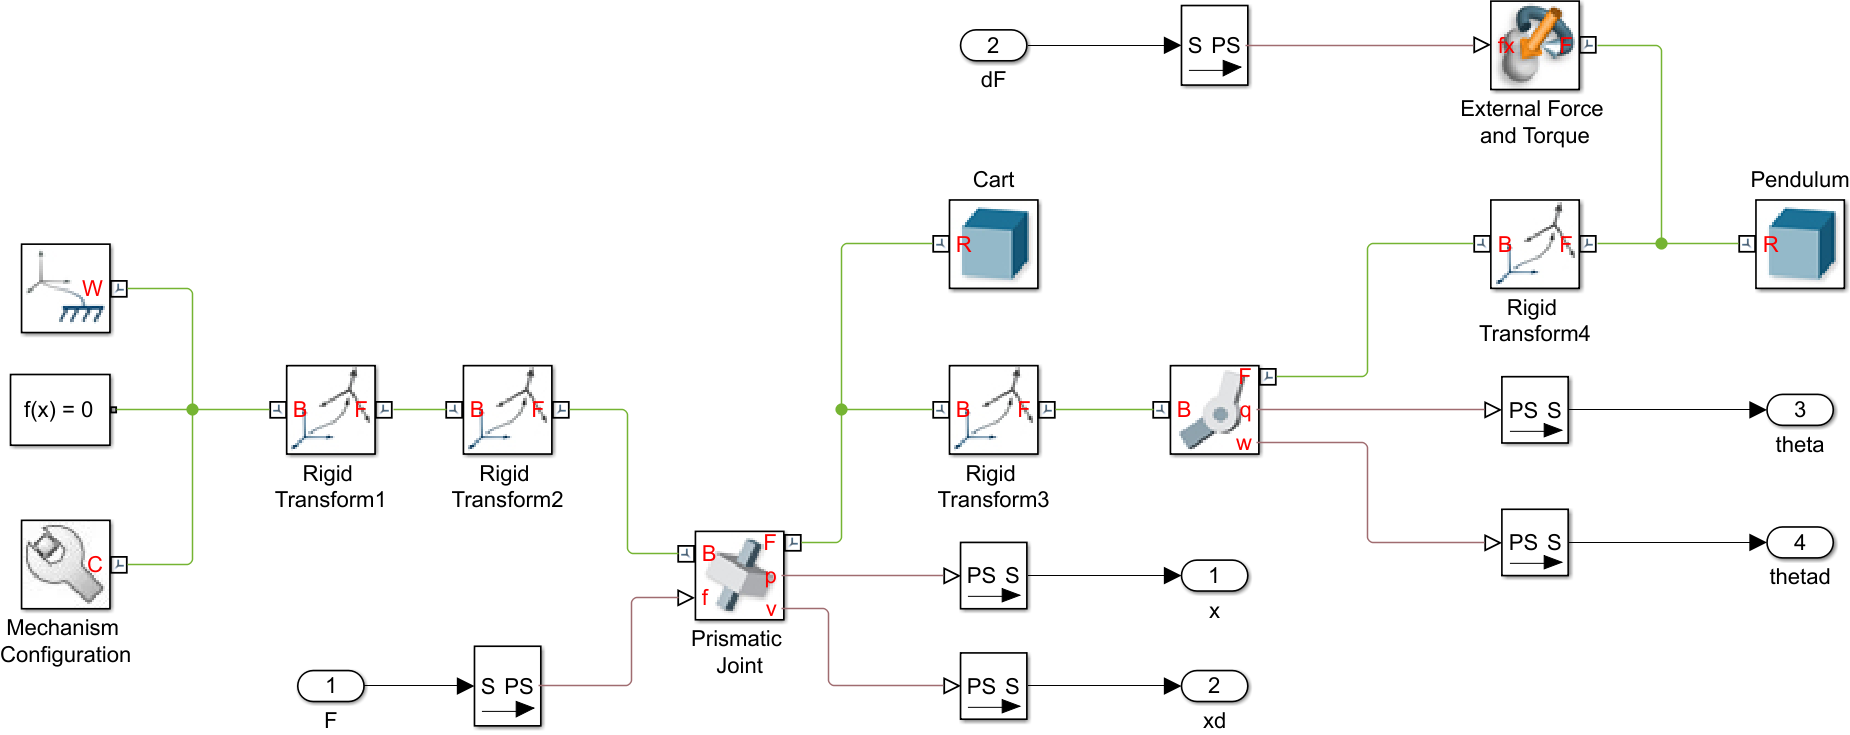
\includegraphics[width=0.9\linewidth]{ImagenesDiseño de Planta/planta_simscape}
	\caption{Planta empleada en Simulink desarrollada con Simscape.}	
	\label{fig:planta_simscape}
\end{figure}

En dicho sistema posee 2 entradas y 4 salidas. Las primeras consisten en la fuerza aplicada al carro (entrada 1 llamada \textit{F}) y un disturbio en el péndulo (entrada 2 denominada \textit{dF}). Por otro lado, las 4 salidas son las variables de estado: posición del carro, velocidad del carro, ángulo del péndulo y velocidad angular del péndulo.

%\end{document}